\documentclass{beamer}
\usepackage[latin1]{inputenc}
\usepackage{times}
\usepackage{tikz}
\usetheme{Luebeck}
%\usecolortheme{albatross}
\usepackage{amsmath,amsfonts,amsthm,amssymb}
\usepackage{setspace}
\usepackage{Tabbing}
\usepackage{fancyhdr}
\usepackage{lastpage}
\usepackage{extramarks}
\usepackage{chngpage}
\usepackage{soul,color}
\usepackage{graphicx,float,wrapfig}
\usepackage{xcolor}
\usepackage{listings}
\usepackage{float}
%\usepackage{subfloat}
\usepackage{subfig}
\usepackage{caption}
\usepackage{enumitem}
\usepackage{algpseudocode}

\definecolor{darkorange}{RGB}{240, 120, 0}
\definecolor{darkgreen}{RGB}{0, 128, 0}

\setbeamercolor{background canvas}{bg=white}
\setbeamercolor{frametitle}{fg=white, bg=darkorange}
\setbeamercolor{normal text}{bg=black,fg=black}
\setbeamercolor{structure}{bg=black, fg=darkorange}


\lstdefinestyle{customc}{
  belowcaptionskip=1\baselineskip,
  breaklines=true,
  frame=L,
  xleftmargin=\parindent,
  language=Python,
  showstringspaces=false,
  basicstyle=\footnotesize\ttfamily,
  keywordstyle=\bfseries\color{green!40!black},
  commentstyle=\itshape\color{purple!40!black},
  identifierstyle=\color{blue},
  stringstyle=\color{orange},
}

\lstdefinestyle{customc}{
  belowcaptionskip=1\baselineskip,
  breaklines=true,
  frame=L,
  xleftmargin=\parindent,
  language=Python,
  showstringspaces=false,
  basicstyle=\footnotesize\ttfamily,
  keywordstyle=\bfseries\color{green!40!black},
  commentstyle=\itshape\color{purple!40!black},
  identifierstyle=\color{blue},
  stringstyle=\color{orange},
}

\lstdefinestyle{customcsmall}{
  belowcaptionskip=1\baselineskip,
  breaklines=true,
  frame=L,
  xleftmargin=\parindent,
  language=Python,
  showstringspaces=false,
  basicstyle=\footnotesize\ttfamily,
  keywordstyle=\bfseries\color{green!24!black},
  commentstyle=\itshape\color{purple!24!black},
  identifierstyle=\color{blue},
  stringstyle=\color{orange},
}

\lstdefinestyle{customcsmall}{
  belowcaptionskip=1\baselineskip,
  breaklines=true,
  frame=L,
  xleftmargin=\parindent,
  language=Python,
  showstringspaces=false,
  basicstyle=\footnotesize\ttfamily,
  keywordstyle=\bfseries\color{green!24!black},
  commentstyle=\itshape\color{purple!24!black},
  identifierstyle=\color{blue},
  stringstyle=\color{orange},
}

\definecolor{MidGreen}{HTML}{00AA00}
\definecolor{MidYellow}{HTML}{AAAA00}

\title{Lecture 15: High Dimensional Data Analysis, Numpy Overview}
\date{3/3/2016}
\institute{Chris Tralie, Duke University}
\author{COMPSCI/MATH 290-04}
\begin{document}

\frame{\titlepage}

\begin{frame}{Announcements}
\begin{itemize}[label=$\vartriangleright$]

\item Mini Assignment 3 Out Tomorrow, due next Friday 3/11 11:55PM

\item Rank Top 3 Final Project Choices By Tomorrow (Groups of 3-4)

\item Dropping Group Assignment 3, Course Grade Schema Change
\begin{itemize}
\item Invidiual And Group Programming Assignments	60\%
\item Final Project	25\%
\item Midterm Exam	5\%
\item Class Participation	5\%
\item Wikipedia Edit	5\%
\end{itemize}

\item Midterm Next Thursday 3/10

\end{itemize}

\end{frame}

\begin{frame}{Table of Contents}
\begin{itemize}[label=$\blacktriangleright$]
	\item Final Project Choices
\end{itemize}
\begin{itemize}[label=$\vartriangleright$]
	\item High Dimensional Data Analysis Intro
\end{itemize}
\begin{itemize}[label=$\vartriangleright$]
	\item Evaluating Classification Performance
\end{itemize}
\begin{itemize}[label=$\vartriangleright$]
	\item Numpy Fundamentals
\end{itemize}
\end{frame}

\begin{frame}{3D Surface Equidecomposability Animation}

\begin{figure}[t]
	\centering
    \includegraphics[width=\textwidth]{FinalProjects/Equidecomposability.png}
\end{figure}

Point Person: Chris Tralie

\end{frame}

\begin{frame}{Ghissi Alterpiece Real Time Rendering}
\begin{figure}[t]
	\centering
    \includegraphics[width=0.8\textwidth]{FinalProjects/Ghissi_Alterpiece.png}
\end{figure}

Point Person: Prof Ingrid Daubechies

\end{frame}


\begin{frame}{Motion Capture Javascript Animation}
\begin{figure}[t]
	\centering
    \includegraphics[width=0.8\textwidth]{FinalProjects/MOCAPData.png}
\end{figure}

Point People: Chris Tralie / (Prof Ingrid Daubechies?)

\end{frame}


\begin{frame}{Blood Vessel Statistics}
\begin{figure}[t]
	\centering
    \includegraphics[width=0.6\textwidth]{FinalProjects/Planes-Pressure.jpg}
\end{figure}

Point People: John Gounley / Prof Amanda Randles

\end{frame}

\begin{frame}{Nasher Museum Talking Heads}
\begin{figure}[t]
	\centering
    \includegraphics[width=0.7\textwidth]{FinalProjects/Nasher.png}
\end{figure}

Point People: Chris Tralie, Prof Caroline Bruzelius

\end{frame}

\begin{frame}{Face Model Fitting / Morphing}
\begin{figure}[t]
	\centering
    \includegraphics[width=0.7\textwidth]{FinalProjects/3DFaceFitting.png}
\end{figure}

Point People: Jordan Hashemi, Qiang Qiu

\end{frame}




\begin{frame}{Table of Contents}
\begin{itemize}[label=$\vartriangleright$]
	\item Final Project Choices
\end{itemize}
\begin{itemize}[label=$\blacktriangleright$]
	\item High Dimensional Data Analysis Intro
\end{itemize}
\begin{itemize}[label=$\vartriangleright$]
	\item Evaluating Classification Performance
\end{itemize}
\begin{itemize}[label=$\vartriangleright$]
	\item Numpy Fundamentals
\end{itemize}
\end{frame}

\begin{frame}{High Dimensional Euclidean Vectors}
For $d$-dimensional vectors

\[ \vec{a} = (a_1, a_2, \hdots, a_d) \]

\[ \vec{b} = (b_1, b_2, \hdots, b_d) \]

\uncover<2->{
Vector addition:

\[ \vec{a+b} = (a_1 + b_1, a_2 + b_2, \hdots, a_d + b_d) \]
}

\uncover<3->{
Vector subtraction:

\[ \vec{ab} = (b_1 - a_1, b_2 - a_2, \hdots, b_d - a_d) \]
}

\end{frame}

\begin{frame}{High Dimensional Euclidean Vectors}
Pythagorean Theorem for

\[ \vec{a} = (a_1, a_2, \hdots, a_d) \]


\[ ||\vec{a}|| = \sqrt{ a_1^2 + a_2^2 + \hdots + a_d^2 } \]

\end{frame}


\begin{frame}{High Dimensional Euclidean Vectors}

Dot product still holds!

\[ \vec{a} \cdot \vec{b} = a_1b_1 + a_2b_2 + \hdots + a_db_d = ||\vec{a}|| ||\vec{b}|| \cos(\theta) \]

Vectors lie on a plane in high dimensions

\end{frame}

\begin{frame}{Histogram Euclidean Distance}

\begin{figure}[t]
	\centering
    \includegraphics[width=0.5\textwidth]{ShapeHist9.pdf}
\end{figure}

For histograms $h_1$ and $h_2$

\[ d_E(h_1, h_2) = \sqrt{ \sum_{i=1}^N (h_1[i] - h_2[i])^2 } \]

Just thinking of $h_1$ and $h_2$ as high dimensional Euclidean vectors!  Each histogram bin is a dimension

\end{frame}

\begin{frame}{Histogram Cosine Distance}

\[ d_C(h_1, h_2) = \cos^{-1}\left(  \frac{ \vec{h_1} \cdot \vec{h_2} }{ ||\vec{h_1}|| ||\vec{h_2}|| } \right) \]

\end{frame}

\begin{frame}{Images Can Be Vectors Too!}

\begin{figure}[t]
	\centering
    \includegraphics[width=0.8\textwidth]{ISOMAP.png}
\end{figure}
\small One axis per pixel.  Above point cloud of images has been flattened to the plane by a nonlinear dimension reduction technique

\tiny J. B. Tenenbaum, V. de Silva and J. C. Langford 

\end{frame}

\begin{frame}{My Work On Video Loops}

\begin{figure}[t]
	\centering
    \includegraphics[width=0.8\textwidth]{VideoStackTime.pdf}
\end{figure}

\small Tralie 2016

\end{frame}

\begin{frame}{My Work On Video Loops}

\begin{figure}[t]
	\centering
    \includegraphics[width=0.6\textwidth]{NeckBeatPCADGMCC.pdf}
\end{figure}

\small Tralie 2016

\end{frame}

%\begin{frame}{Euclidean Distance Shortcomings}

%\begin{figure}[t]
%	\centering
%    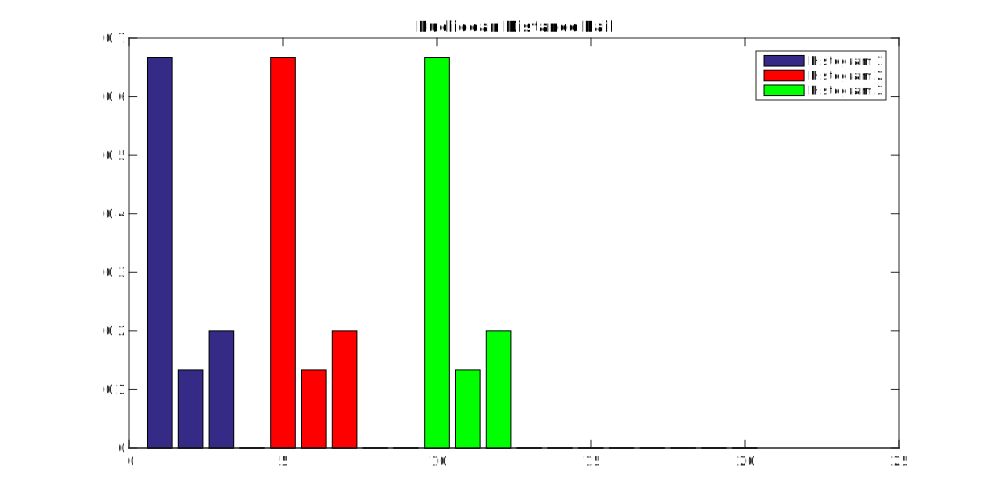
\includegraphics[width=\textwidth]{EuclidHistFail.pdf}
%\end{figure}

%They all have the same distance!

%\end{frame}


%\begin{frame}{Euclidean Distance Shortcomings}

%\begin{figure}[t]
%	\centering
%    \includegraphics[width=\textwidth]{EMDVisual.pdf}
%\end{figure}

%Move earth from blue to red

%\end{frame}

%\begin{frame}{Earth Mover's Distance}

%\begin{figure}[t]
%	\centering
%    \includegraphics[width=0.8\textwidth]{1DEMDExample.png}
%\end{figure}

%\end{frame}

%\begin{frame}{Chi Squared Distance}

%\[ d_{\chi}(h_1, h_2) = \frac{1}{2} \sum_{i=1}^N \frac{(h_1[i] - h_2[i])^2}{h_1[i]+h_2[i]}\]

%Exclude values for which $h_1[i] = h_2[i] = 0$

%\end{frame}


%\begin{frame}{Normalize Histograms By Mass}

%\[ h'[i] = \frac{h[i]}{\sum_{k=1}^N h[k]} \]

%In other words, all bins should sum to 1

%\end{frame}


\begin{frame}{Table of Contents}
\begin{itemize}[label=$\vartriangleright$]
	\item Final Project Choices
\end{itemize}
\begin{itemize}[label=$\vartriangleright$]
	\item High Dimensional Data Analysis Intro
\end{itemize}
\begin{itemize}[label=$\blacktriangleright$]
	\item Evaluating Classification Performance
\end{itemize}
\begin{itemize}[label=$\vartriangleright$]
	\item Numpy Fundamentals
\end{itemize}
\end{frame}



\begin{frame}{Evaluation Strategy}

Do {\em leave one out} technique

\begin{itemize}

\item Use each item as test item in turn, compare to database

\end{itemize}

\begin{itemize}[label=$\blacktriangleright$]

\item Summarize evaluation statistics over entire database by {\em averaging them}

\end{itemize}

\end{frame}

\begin{frame}{Precision / Recall}

\begin{figure}[t]
	\centering
    \includegraphics[width=\textwidth]{PrecisionRecall.png}
\end{figure}

Rusinkiewiz/Funkhouser 2009

\end{frame}

\begin{frame}{Other Evaluation Metrics}

\begin{itemize}[label=$\vartriangleright$]

\item Average Precision (Area Under Precision/Recall Curve)

\item Mean Reciprocal Rank (1/rank of first correct item)

\item Median Reciprocal Rank

\end{itemize}

1 is perfect score

\end{frame}


\begin{frame}{Table of Contents}
\begin{itemize}[label=$\vartriangleright$]
	\item Final Project Choices
\end{itemize}
\begin{itemize}[label=$\vartriangleright$]
	\item High Dimensional Data Analysis Intro
\end{itemize}
\begin{itemize}[label=$\vartriangleright$]
	\item Evaluating Classification Performance
\end{itemize}
\begin{itemize}[label=$\blacktriangleright$]
	\item Numpy Fundamentals
\end{itemize}
\end{frame}

\begin{frame}{Python for This Class}

\begin{itemize}[label=$\vartriangleright$]
\item Use Python 2.7
\item Switch your editor to use 4 spaces per tab instead of tabs (!!)
\item Required Packages: numpy, matplotlib, pyopengl, wxpython
\item Optional Packages: scipy (for some extra tasks)
\item Helpful Interactive Code Editing: ipython
\end{itemize}

\end{frame}

\begin{frame}{Python Basics}

\lstinputlisting[style=customc]{NumpyDemos/pybasics.py}

\end{frame}

\begin{frame}{Numpy: Array Basics}

Numpy = Python + Matlab

\lstinputlisting[style=customc]{NumpyDemos/npbasics.py}

\end{frame}


\begin{frame}{Numpy: Randomly Subsample}

\lstinputlisting[style=customc]{NumpyDemos/randsubsample.py}

\end{frame}


\begin{frame}{Numpy: Boolean Distance Select}

\lstinputlisting[style=customc]{NumpyDemos/distselect.py}

\end{frame}


\begin{frame}{Numpy: Boolean Distance Select}

\lstinputlisting[style=customc]{NumpyDemos/distselect.py}

\end{frame}

\begin{frame}{Numpy: Broadcasting, Rotate Ellipse}

\lstinputlisting[style=customc]{NumpyDemos/rotateellipse.py}

\end{frame}


\begin{frame}{Numpy: Broadcasting, Sphere Normalization}

\lstinputlisting[style=customc]{NumpyDemos/spherenorm.py}

\end{frame}

\begin{frame}{Numpy: More Broadcasting}

\lstinputlisting[style=customc]{NumpyDemos/broadcasting.py}

\end{frame}

\begin{frame}{Numpy: PCA Implementation}

\lstinputlisting[style=customcsmall]{NumpyDemos/pcademo.py}

\end{frame}

\begin{frame}{Squared oooEuclidean Distances in Matrix Form}
Notice that

\[ ||\vec{a} - \vec{b}||^2 = (\vec{a} - \vec{b}) \cdot (\vec{a}-\vec{b}) \]

\[ ||\vec{a} - \vec{b}||^2 = \vec{a} \cdot \vec{a} + \vec{b} \cdot \vec{b} - 2 \vec{a} \cdot \vec{b} \]

\uncover<2->{

Given points clouds $X$ and $Y$ expressed as $2 \times M$ and $2 \times N$ matrices, respectively, write code to compute an $M \times N$ matrix $D$ so that

\[ D[i, j] = ||X[:, i] - Y[:, j]||^2 \]

Without using any for loops!  Can use for ranking with Euclidean distance or D2 shape histograms, for example

}

\end{frame}

\begin{frame}{Brute Force Nearest Neighbors}

\lstinputlisting[style=customcsmall]{NumpyDemos/NearestNeighborBrute.py}

\end{frame}

\end{document}

